\documentclass[11pt, a4paper]{ECON2123}
\usepackage{verbatim}
\usepackage{fancyhdr}
\usepackage{booktabs}
\usepackage{setspace}
\usepackage{amsmath,mathrsfs}
\usepackage{multicol}
\usepackage{amssymb}
\usepackage{graphicx}
\usepackage{caption}
\usepackage{subcaption}
\usepackage{array}
\usepackage{xcolor}
\usepackage{float}
\usepackage{enumitem}
\usepackage{mathcomp}
\usepackage{tabularx}
\usepackage{wasysym}
\usepackage{pbox}
\usepackage{tikz}
\usepackage{mathtools}
\usetikzlibrary{matrix}
\usepackage[normalem]{ulem}
\usepackage{multirow}
\usepackage[linesnumbered, ruled, boxed]{algorithm2e}
\SetKwRepeat{Do}{do}{while}

\title{Chapter 01 \& 02}
\subtitle{Basics}

\begin{document}
\begin{spacing}{1.5}
    
    \section{Overall introduction}

    {\bf How can we describe an economy?}
    \begin{itemize}
        \item Output
        \item Unemployment rate
        \item Inflation rate
    \end{itemize}
    
    {\bf How the crisis happened?} 
    \begin{itemize}
        \item Housing market $\rar$ whole financial system. 
        How such a small part of financial system affected an 
        entirely system? Nearly the whole US finance.
        \item How from financial sector $\rar$ real-side economy?
        \item How from US domestic $rar$ world-wide crisis? The great depression 
        confined in US, but why 2008 crisis affected all over the world?
    \end{itemize}

    {\bf Why China {\it seemed} to be intact in 2008 Financial Crisis?}

    The adverse effect on demand was nearly fully offset by 
    a major fiscal expansion by Chinese government. 
    (a major increase in public investment)


    \section{GDP: ``Aggregate Output''}

    \subsection{Measure GDP}

    {\bf GDP: G}ross {\bf D}omestic {\bf P}roduct

    \begin{itemize}
        \item Gross: we care about the whole, total, aggregate value, 
        not individually.
        \item Domestic: as long as in the region, no matter who produce,
        differ from ``GNP''
        \item Product: care about output.
    \end{itemize}

    How to measure? By {\bf national income and product accounts}, 
    which is an accounting system to measure aggregate economic activity.

    Example: 
    \begin{center}
        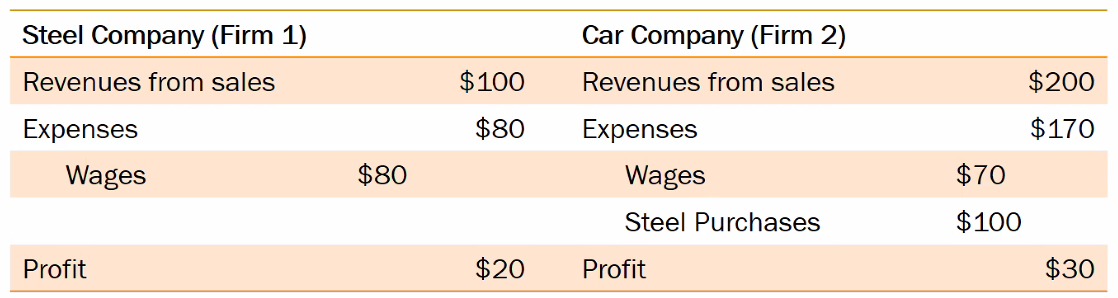
\includegraphics[scale=0.8]{images/0102-GDP-1.png}
    \end{center}
    How to calculate GDP? 
    $300=100+200$? This double counts {\bf intermediate} goods.
    $50=20+30$? This is profit income, not total output, which 
    underestimate the total output.
    \begin{itemize}
        \item Only care about value of {\bf final goods.} 
        Just the revenues of the car: $200$.
        Final goods aim for {\bf final consumption.}
        \item Value {\bf added} in the company.(like contributions)
        $100+(200-100)=200$, since in company 2, it add 
        100 to make steel into cars.
        \item Income side: income for workers(labor income) + 
        income for company(profit income).
        $80+20+70+30=200$.
    \end{itemize}

    Someone buy a piece of fish for eat, the fish is a {\bf final good},
    but if he cook it and sell it to his neighbor, then it will 
    become an {\bf intermediate} good.

    In summary, we can calculate GDP from two sides, in three ways:

    {\bf Production side:}
    \begin{itemize}
        \item the value of the {\bf final} goods and services produced in 
        the economy during a given period.
        \item the sum of {\bf value added} in the economy during a given period.
    \end{itemize}

    {\bf Income side:}
    \begin{itemize}
        \item the sum of {\bf incomes} in the economy during a given period.
    \end{itemize}

    During a given period, {\bf aggregate production = aggregate income.}

    Quiz: A firm's value added equals 
    {\it {its revenue minus its cost of intermediate goods.}}
    A firm's profit equals {\it {its revenue minus its costs.}}

    \subsection{nominal \& real GDP}

    {\bf nominal: } in current price, {\bf real:} in a fixed price,
    more like in quantity.

    Nominal GDP not only captures the changes in {\bf product capacity},
    but also captures the changes in {\bf prices}(inflation).
    \begin{center}
        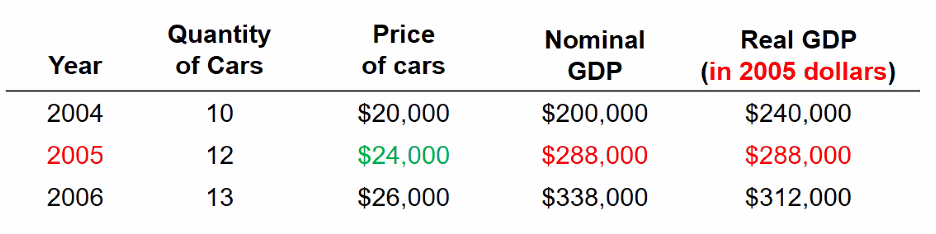
\includegraphics[scale=0.8]{images/0102-nominal-real-gdp.png}
    \end{center}
    However, real GDP doesn't show us the improvement of quality:
    a 1990 car has the same price as a latest car.
    To account for that, we use ``Hedonic pricing'', where 
    instead of focusing on the car as a whole, we break it 
    into parts and evaluate the improvements individually.
    (refer to ch2 focus box)

    Another problem: why do we use real GDP, rather then directly 
    use the quantity of things we make as the GDP number?
    For example, economy $A$ produces 100 planes and 1 car, while $B$
    produces 1 plane and 100 cars. Which one is more powerful?
    $P\times Q$ suggests that country that makes more planes are 
    more powerful than the one makes more cars.

    More than one good, real GDP is a {\bf weighted average} 
    of the output of all final goods, and {\bf relative prices}
    determine the weights, which change over time!
    So this weights actually reflect relative prices 
    and {\bf changes over time.}
    The measure is called {\bf real GDP in chained(2005) dollars.} (refer to ch2 
    appendix)

    \subsection{GDP level \& growth rate}

    \begin{itemize}
        \item {\bf the level of real GDP:} gives the economic 
        size of a country.
        \item {\bf real GDP per person:} standard of living of the country.
        \item {\bf GDP growth:} $\dfrac{Y_t-Y_{t-1}}{Y_{t-1}}$ for {\bf real} GDP.
    \end{itemize}

    Periods of negative GDP growth are called {\bf recessions},
    positive growth are called {\bf expansions.}

    
    \subsection{useful?}

    What can be measured in GDP?
    \begin{itemize}
        \item Goods and services available for consumption
        \item Consumers' {\bf valuation} on these items.
        \item {\it A good measure of the material life??}
    \end{itemize}

    What cannot be measured in GDP?
    \begin{itemize}
        \item Goods and services without {\bf market prices}:
        government services, owner-occupied housing etc.
        \item Goods and services {\bf not traded} in markets:
        leisure, housework
        \item depletion of natural and environmental resources.
    \end{itemize}

    Actually, GDP or its rate cannot precisely reflect the living 
    standard of a country/region. Like the data of Macau as shown below.
    Therefore, unemployment rate is introduced.
    \begin{center}
        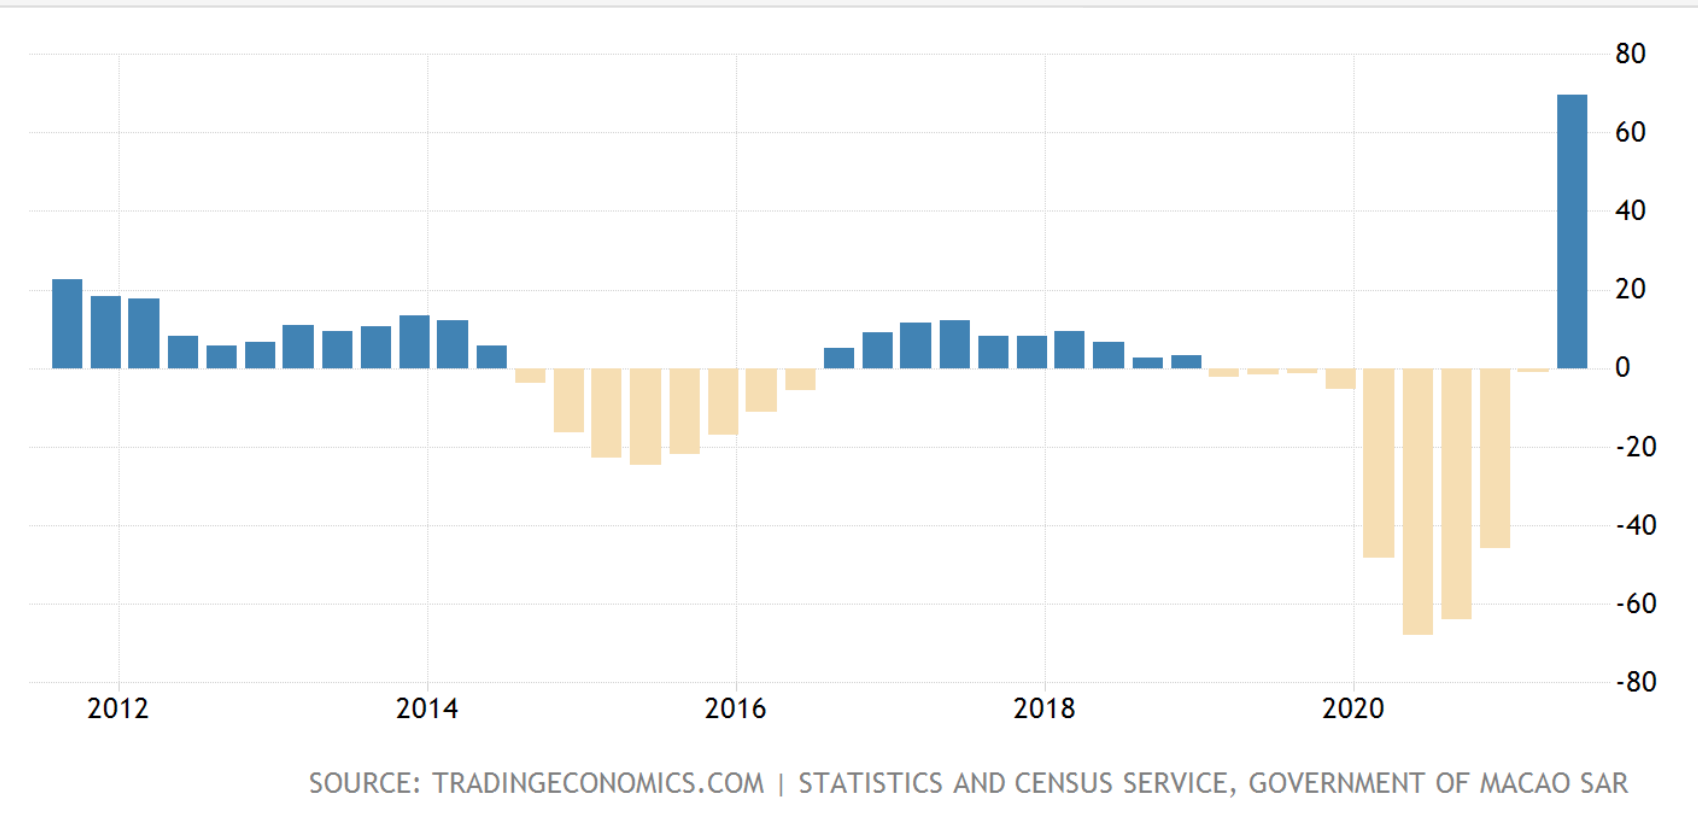
\includegraphics[scale=0.4]{images/0102-macau-gdp.png}
    \end{center}

    {\it Yet the gross national product does not allow for the health of 
    our children, the quality of their education or the joy of their play. 
    It does not include the beauty of our poetry or the strength of our marriages, 
    the intelligence of our public debate or the integrity of our public officials. 
    It measures neither our wit nor our courage, neither our wisdom nor our learning, 
    neither our compassion nor our devotion to our country, it measures everything 
    in short, except that which makes life worthwhile.}
    \begin{flushright}
        —— Robert F. Kennedy
    \end{flushright}

    \section{Unemployment Rate}

    \begin{itemize}
        \item {\bf employment:($N$) } the number of people who have a job
        \item {\bf unemployment:($U$) } the number of people who do not 
        have a job but {\bf are looking for one.} (those who do not have a 
        job and are not looking for one are counted as {\bf not in the labor force})
        \item {\bf labor force:($L=N+U$) } sum of employment and unemployment.
        \item {\bf unemployment rate: } $u=\dfrac{U}{L}$
        \item {\bf participation rate: } 
        $=\dfrac{L}{total\ population\ of\ working\ age}$.
    \end{itemize}

    However, this number is hard to calculate, since it's difficult
    to decide whether someone is ``looking for a job''.
    US uses a survey called Current Population Survey (CPS) 
    and classify a person as ``unemployed'' if he or she does not 
    have a job and {\it has been looking for a job in the last four weeks.}

    When the economy slows down, we typically observe both an 
    {\bf increase in unemployment} and an {\bf increase in the number of people 
    who drop out of the labor force(lower participation rate)}. 

    {\bf Why unemployment rate is important?}
    \begin{itemize}
        \item has direct effect on the welfare of the unemployed: 
        if unemployment increases, it becomes more {\bf widespread} 
        and more {\bf painful}.
        {\bf Discouraged workers: } without jobs who give up looking 
        for work.(low partic rate)
        \item it provides a signal that the economy may not be 
        using some of its resources efficiently
    \end{itemize}

    \section{Inflation Rate}

    \begin{itemize}
        \item {\bf inflation}: a sustained rise in the general level of {\bf prices} 
        ({\bf price level})
        \item {\bf deflation}: a sustained decline in the price level
        \item {\bf inflation rate}: the rate at which the price level increases.
    \end{itemize}

    Usually there are two measures of price level: ({\bf two price indexes})
    \begin{itemize}
        \item the {\bf GDP deflator}
        \item the {\bf Consumer Price Index}
    \end{itemize}

    \subsection{GDP deflator}

    If we see nominal GDP increase faster than real GDP, the difference 
    must come from an {\bf increase in prices.} This motivates the 
    definition of the GDP deflator.
    $$P_t=\frac{\text{Nominal GDP}_t}{\text{Real GDP}_t}=\frac{\$ Y_t}{Y_t}$$

    The GDP deflator is called an {\bf index number}. Its level has no economic 
    interpretation. But its rate of change, $\pi_t=\dfrac{P_t-P_{t-1}}{P_{t-1}}$, 
    has a clear economic interpretation: It gives the rate at which the general 
    level of prices increases over time: i.e., {\bf the rate of inflation.}

    Moreover, this also implies a simple relation among nominal GDP, 
    real GDP, and the GDP deflator:
    $$\$Y_t = P_t\cdot Y_t$$
    Thus, the {\bf rate of growth of nominal GDP} is equal to the 
    {\bf rate of inflation} plus the {\bf rate of growth of real GDP}.

    \subsection{Consumer Price Index}

    The GDP deflator gives the average price of {\bf output}: the final 
    goods produced in the economy. But consumers care about the average 
    price of {\bf consumption}: the goods they consume. 
    The two prices need not be the same: The set of goods produced 
    is not the same as the set of goods purchased by consumers:
    \begin{itemize}
        \item Some goods in GDP are sold not to consumers but to 
        firms/government/foreigners.
        \item Some goods bought by consumers are imported from abroad.
    \end{itemize}

    To measure the average price of {\bf consumption}, or, equivalently, 
    the {\bf cost of living}, we look at {\bf the Consumer Price Index(CPI)}.
    \begin{center}
        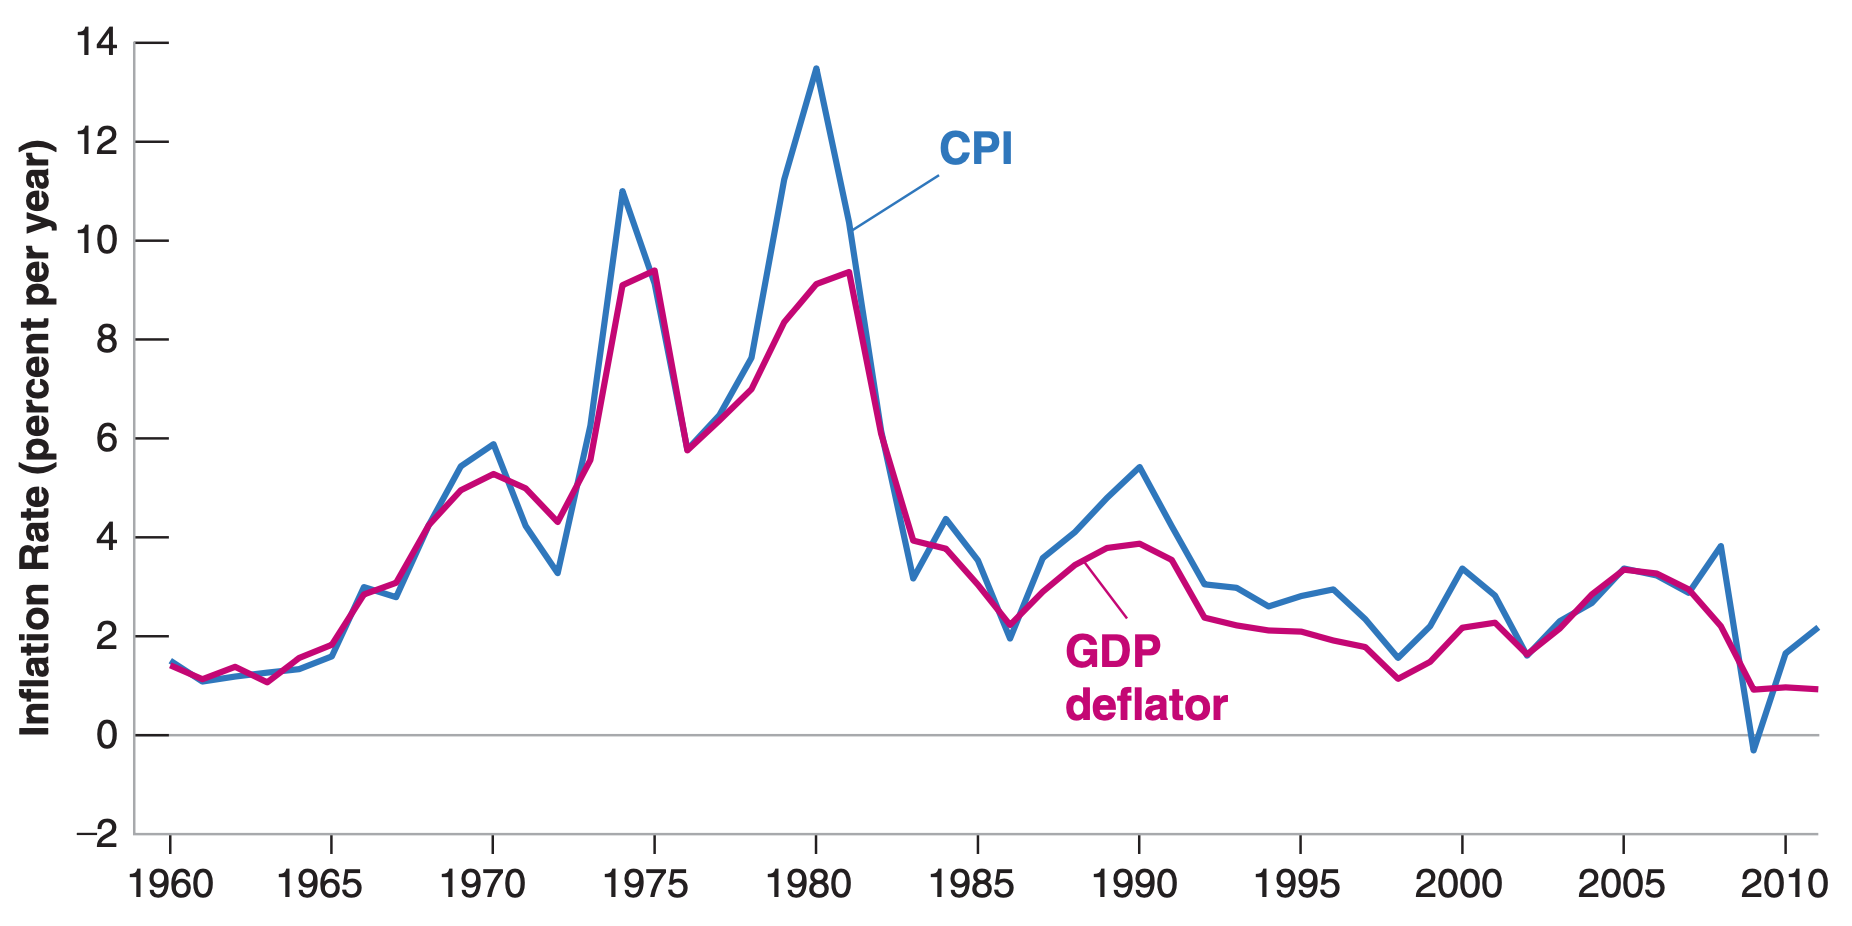
\includegraphics[scale=0.36]{images/0102-cpi-vs-deflator.png}
    \end{center}
    \begin{itemize}
        \item The CPI and the GDP deflator {\bf move together} most of the time.
        \item Exceptions: GDP deflator is the price of goods {\it produced}, 
        whereas the CPI is the price of goods {\it consumed}.
    \end{itemize}

    {\bf Why inflation rate is important?}

    If a higher inflation rate meant just a faster but {\bf proportional} 
    increase in all prices and wages(pure inflation), inflation would be 
    only a minor inconvenience, as {\bf relative prices would be unaffected}.

    However, this is not the case:
    \begin{itemize}
        \item not all prices and wages rise proportionately. e.g. retirees.
        \item inflation leads to other distortions. e.g. firms more uncertain 
        about future investment; bracket creep: higher tax.
    \end{itemize}

    But what about deflation?

    We expect the price to be lower and lower in the future, 
    so we just wait, instead of buying it now. 
    Firms, also, lose motivations to buy machines, and 
    their goods are cheaper and cheaper, therefore have 
    no incentives to improve, don't want to make investment.
    All those cause a {\bf worse} economy.

    \section{Okun's Law}

    {\bf negative} relationship between {\bf GDP growth}
    and {\bf change in unemployment rate}. 
    (if output growth is high, unemployment will decrease)
    \begin{center}
        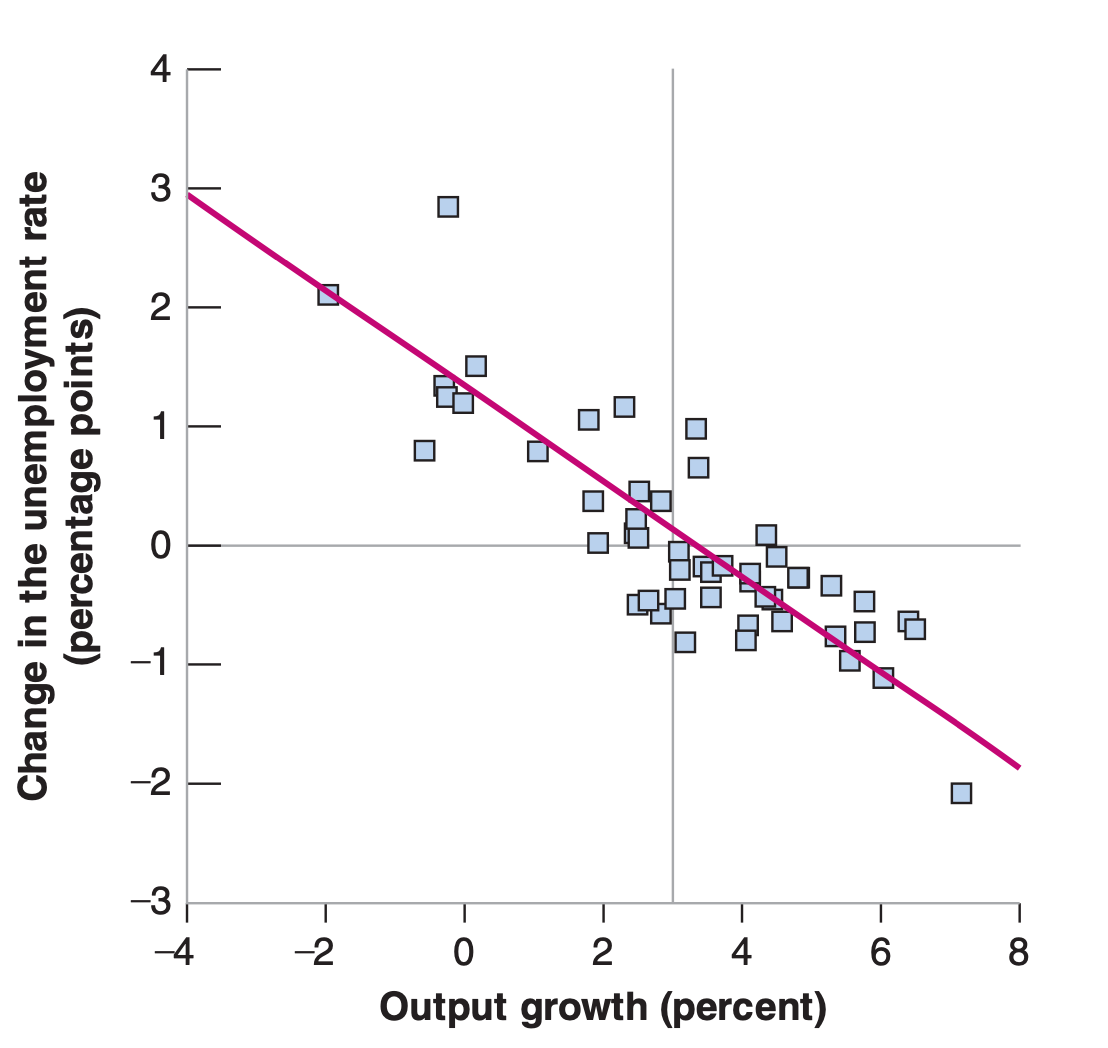
\includegraphics[scale=0.3]{images/0102-okun-law.png}
    \end{center}

    This vertical line crosses the horizontal axis at the 
    point where output growth is roughly equal to 3\%: 
    It takes a growth rate of about 3\% to keep unemployment 
    constant. Two reasons:
    \begin{itemize}
        \item population, thus labor force, increase over time.
        \item output per worker is also increasing with time,
        implies that output growth is higher than employment growth.
    \end{itemize}

    \section{The Phillips Curve}

    {\bf negative} relationship between {\bf unemployment rate}
    and {\bf change in inflation rate}. 
    (when unemployment becomes very low, the economy is likely 
    to overheat, and that this will lead to upward pressure 
    on inflation.)
    \begin{center}
        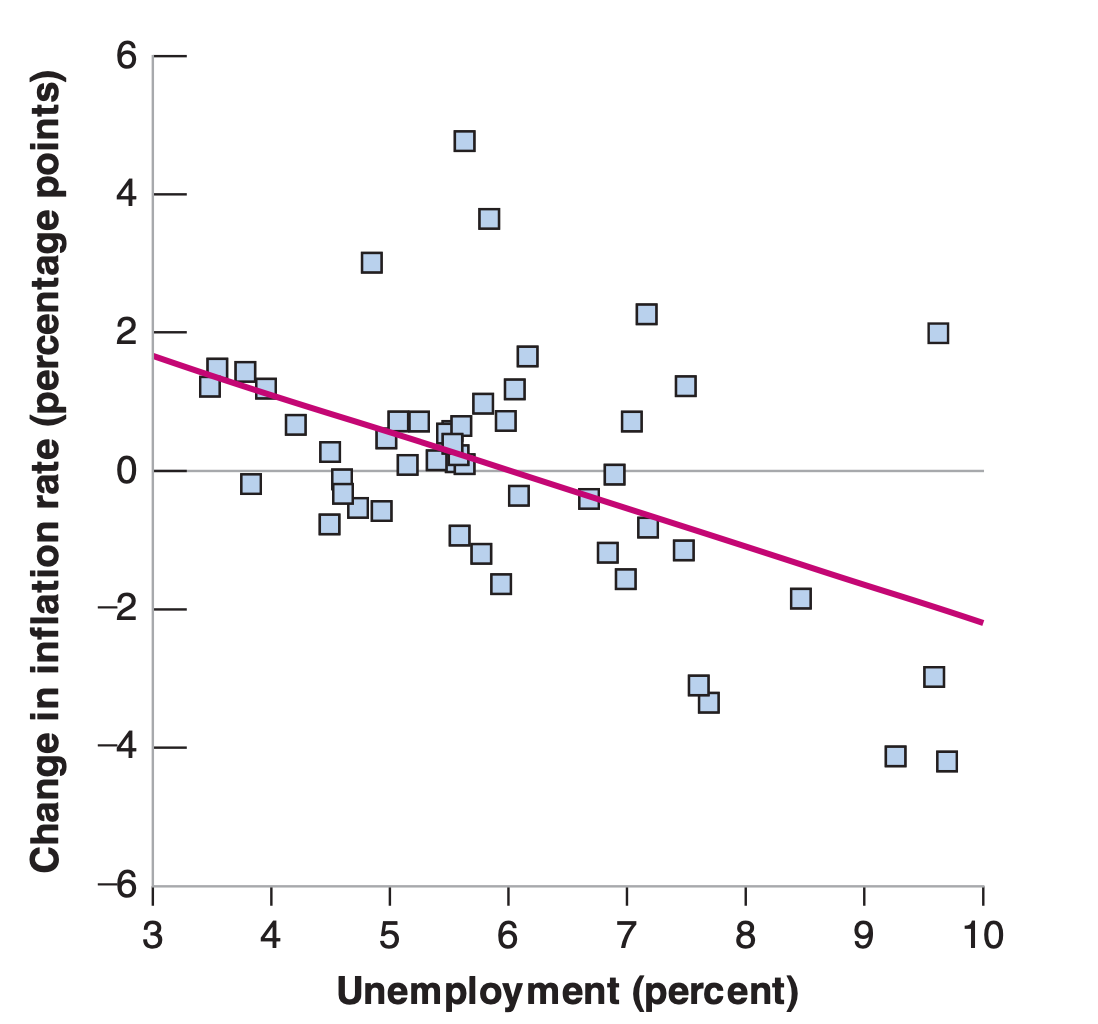
\includegraphics[scale=0.3]{images/0102-phillips-curve.png}
    \end{center}

    When unemployment has been below 6\%, inflation has 
    typically increased, suggesting that the economy was 
    {\bf overheating}, operating above its potential. 

    Notice, this curve is not always true, there are exceptions.

    \section{Time Frame For Determination of Output}
    \begin{itemize}
        \item {\bf Short run:} a few years, changes in output 
        mainly driven by changes in {\bf demand}.
        \item {\bf Medium run:} a decade, output determined 
        by {\bf given supply factors} such as capital stock, 
        technology, size and skills of labor force.
        \item {\bf Long run:} a few decades or more, 
        determined by {\bf changes in supply factors} such as 
        accumulation of capital, tech growth, education, 
        role of government etc.
    \end{itemize}


    {\it This is the end of lecture note. Last modified: Sep 13.\\
    Sep 9: add details after class.\\
    Sep 13: add the section ``Time Frame For Determination of Output''}

\end{spacing}
\end{document}
